\documentclass[tikz,border=7pt]{standalone}
\begin{document}
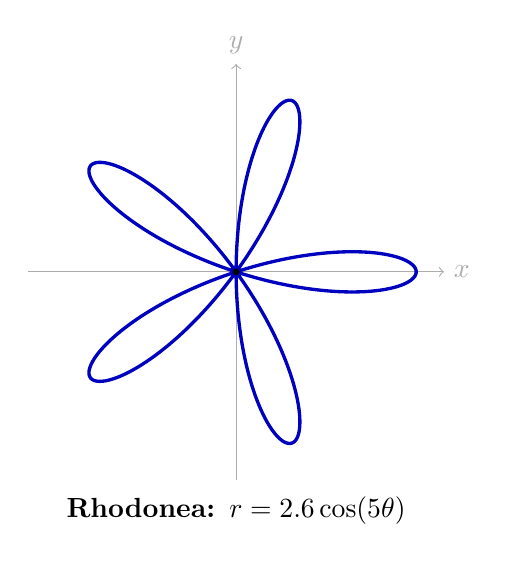
\begin{tikzpicture}[scale=.88]
\draw[->,gray!65] (-3,0)--(3,0) node[right] {$x$};
\draw[->,gray!65] (0,-3)--(0,3) node[above] {$y$};
\draw[blue!75!black,very thick,samples=500,domain=0:360,smooth,variable=\t]
  plot ({2.6*cos(5*\t)*cos(\t)},{2.6*cos(5*\t)*sin(\t)});
\fill (0,0) circle (1.4pt);
\node[font=\bfseries] at (0,-3.45) {Rhodonea: $r=2.6\cos(5\theta)$};
\end{tikzpicture}
\end{document}
